\documentclass{article}

\usepackage{color}
\usepackage{graphicx}
\usepackage{tabularx}
\usepackage[frenchb]{babel}
\usepackage[utf8]{inputenc}
\usepackage[T1]{fontenc}
\usepackage{lmodern}


\usepackage{geometry,wrapfig,lipsum}
 \geometry{
 top=20mm,
 bottom=20mm,
 }


\title{Document pour l'adapation des interfaces}
\author{Justal Kevin}
\date{28/09/2015}
\renewcommand{\contentsname}{Table des mati\`eres} 
 
\newcommand\invisiblesection[1]{%
  \refstepcounter{section}%
  \addcontentsline{toc}{section}{\protect\numberline{\thesection}#1}%
  \sectionmark{#1}} 
 
\begin{document}

\begin{center}
\textbf{\Huge{JEU DES COULEURS}}
\line(1,0){300}\\
ANALYSE ET TEST APPROFONDIS\\
\vspace{3cm}
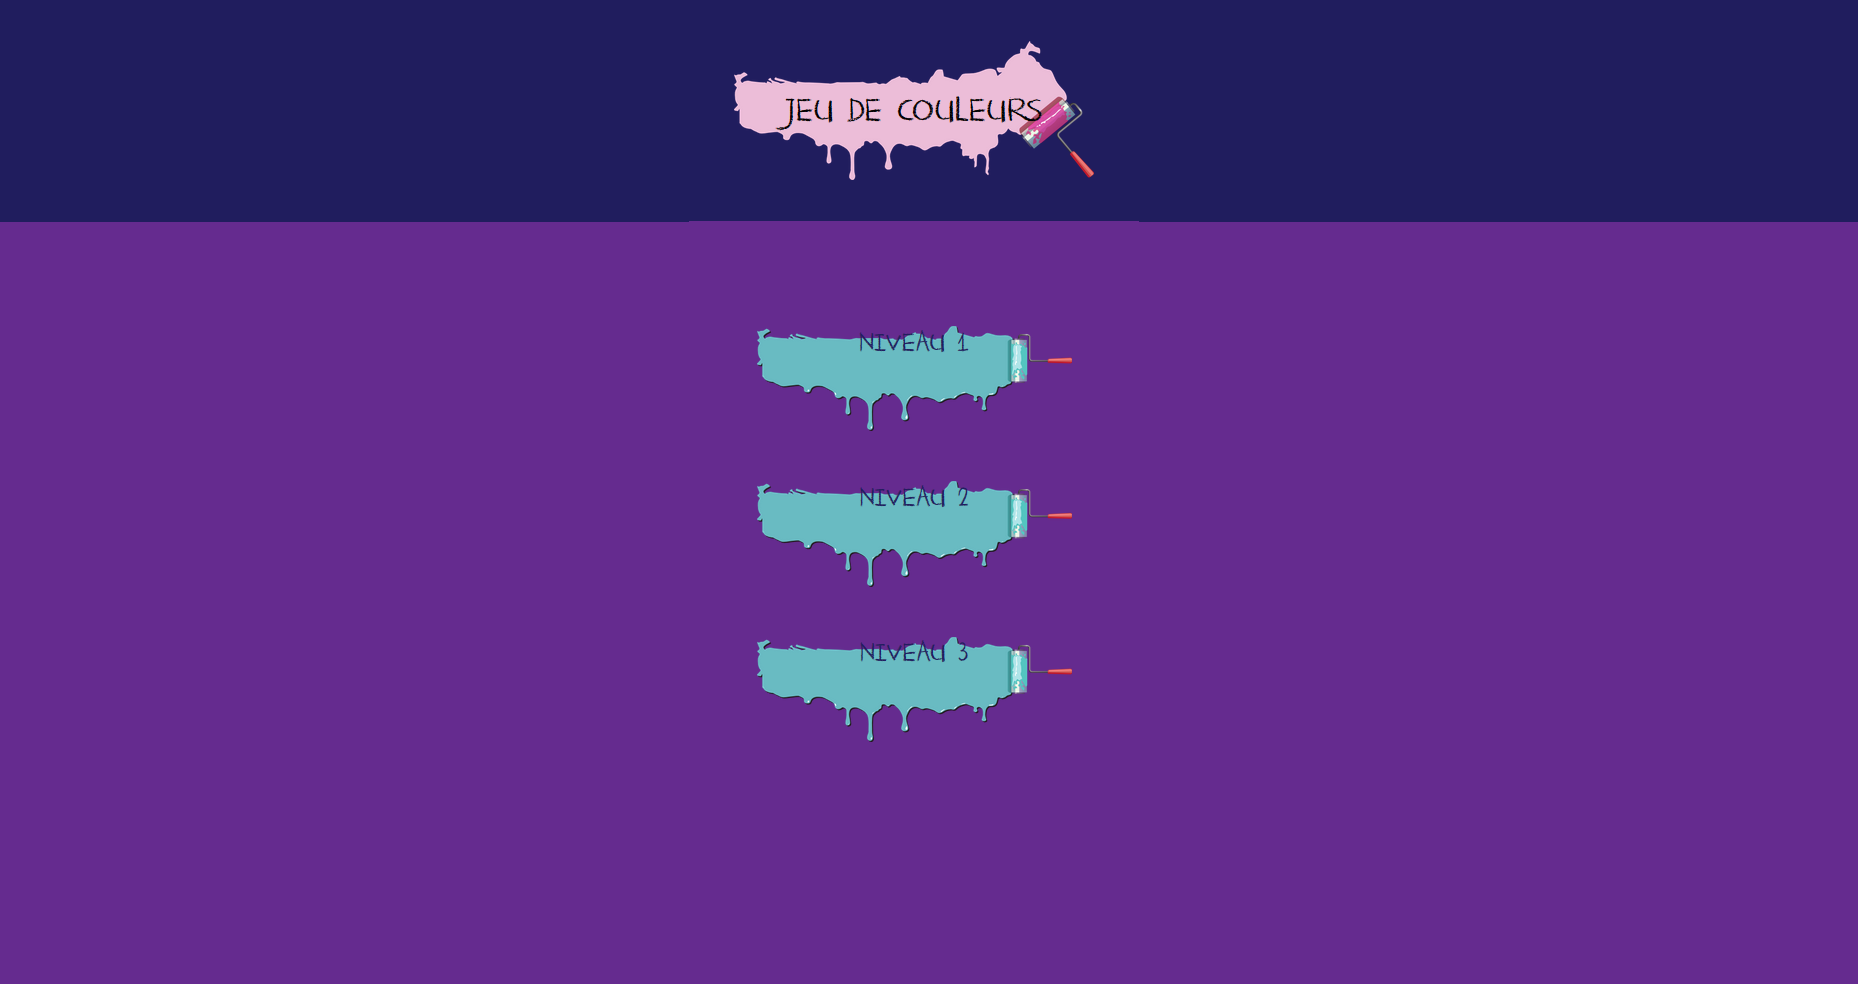
\includegraphics[width=\textwidth]{2}\\
\vspace{3cm}
\textbf{\Large{JUSTAL KEVIN}}\\
2015\\
\vspace{2cm}
\textbf{Justal Kevin - \color{blue}{\underline{justal@polytech.unice.fr}} \color{black}{- SI5 - IHM}}\\
\vspace{4cm}
\textbf{Enseignant :}\\
\textbf{Jean-Paul Stromboni - \color{blue}{\underline{strombon@polytech.unice.fr}}}
\end{center}

\newpage
\tableofcontents

\newpage

\section{Le Jeu}

Le "jeu de couleur" est un jeu très simple basé uneiquement sur les 3 couleurs suivantes : bleu, rouge, jaune. Il dispose de trois niveaux :\\
\begin{itemize}
\item Niveau 1 : Un niveau où le jeu joue à notre place pour montrer le but du jeu.
\item Niveau 2 : Un niveau où il faut reproduire soit même ce que l'on a vue au premier niveau.
\item Niveau 3 : Un niveau où il faut choisir un pot de couleur en fonction de la couleur écrite.
\end{itemize}
\vspace{0.4cm}

Chaque niveau à la même interface graphique. Le fond est blanc. Il y a un bouton "retourner" dans le coin haut gauche en vert puis on retrouve nos pots de peinture posé sur une bande noire.

Le niveau 1 est un niveau de démonstration. Lorsque l'on arrive sur ce niveau, il y a 3 tâches de couleur en haut de la fenêtre et 3 pots de peinture en bas de la fenêtre qui sont placé aléatoirement. Au bout de quelques secondes, une animation se lance et chacune des tâches de couleur se déplacent vers leurs pots de peintures d'origine. Les tâches de couleurs se déplacent les unes après les autres, dans l'ordre de gauche et à droite.\\

Le niveau 2 est identique au précédent. C'est à dire que l'on retrouve bien nos 3 tâches de peinture en haut ainsi que nos trois pots de peinture en bas de la fenêtre. Cette fois-ci le regroupement des tâches en fonction des couleurs est laissé au joueur. Le joueur a deux moyens pour associer les éléments. Soit il clique sur la tâche de peinture puis sur le bon pot correspondant à cette dernière ou soit il clique et maintient le clique pour déplacer la tâche de peinture jusqu'au pot correspondant. Dans le cas d'une bonne association, un son ainsi qu'un signe vert s'affiche et la tâche de peinture devient insaisissable. En cas de mauvaise réponse, un son différent que lorsque la réponse est juste est joué et un signe rouge est affiché à l'écran. La tâche retourne dans ce cas là à sa place originelle.\\

Le niveau 3 est très différent des autres niveaux. Dans ce niveau, il n'y a que 2 pots de peinture et un mot affiché qui est une couleur écrite en toutes lettres en noire. Le joueur doit simplement lire le mot et cliquer ensuite sur la couleur correspondante. En cas de bonne réponse, un son est joué et un signe vert est affiché puis on passe au niveau suivant. Dans le cas contraire, un signe rouge est affiché et le joueur est amené à choisir un nouveau pot de peinture.


\section{Qualités}

\vspace{0.5cm}

\includegraphics[width=\textwidth]{4}\\
\hspace*{0.6cm}La qualité du jeu réside dans son gameplay très simple et intuitif. Il n'y rien d'extravagant sur l'écran qui perturberait le joueur. Il y a juste le minimum requis pour que le jeu soit jouable, c'est à dire 3 couleurs, 3 pots de peinture et 3 tâches de peinture. On comprend donc très vite le principe du jeu. Les t\^aches doivent être associer aux pots de peinture en fonction de leurs couleurs. Un autre bon point pour le jeu est la vitesse d'exécution du programme ainsi que le peu de ressources utilisés. Le jeu doit charger environs 280,83 ko, ce qui est une valeur relativement faible pour un jeu.\\

\begin{wrapfigure}{l}{0.2\textwidth}
  \vspace{-20pt}
  \begin{center}
    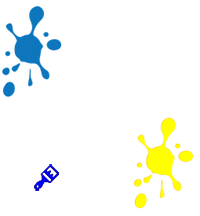
\includegraphics[width=0.18\textwidth]{10}
  \end{center}
  \vspace{-20pt}
  \caption{Le curseur du drag and drop}
  \vspace{-10pt}
\end{wrapfigure}

La prise en main est simple. Il y a deux manières de manipuler les tâches de peinture. De manière classique, on peux effectuer simplement un glisser-déposer. On prend la t\^ache de peinture puis on la déplace dans le pot correspondant. Mais j'ai appris lors de ma visite à l'IME (Institute Médico Educatif) Hirondelles de Biot que les utilisateurs avaient généralement du mal à garder le clic appuyé. C'est pourquoi je suppose que l'on retrouve dans le jeu, une deuxième manière d'effectuer la même opération en cliquant sur la tâche puis sur le pot de peinture. Ceci est une très bonne idée que je vais sans doute reprendre pour mon propre projet si le temps me le permet. Cela permet de s'adapter de manière efficace aux handicaps des enfants.\\

\begin{wrapfigure}{r}{0.2\textwidth}
  \vspace{-20pt}
  \begin{center}
    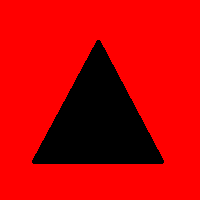
\includegraphics[width=0.18\textwidth]{5}
  \end{center}
  \vspace{-20pt}
  \caption{Symbole lorsque l'on perd}
  \vspace{-10pt}
\end{wrapfigure}

Les résultats du joueur sont aussi très bien signalé dans le jeu. C'est à dire lorsque le joueur donne une bonne réponse ou une mauvaise réponse. Lorsque le joueur triomphe du jeu ou perd, un symbole visuel apparait et un son est joué. En cas de bonne réponse, un rond blanc sur fond vert est affiché et un son de victoire est joué. En cas de mauvaise réponse, un triangle noir sur un fond rouge est affiché et un son de mauvaise réponse est joué. Cela est une excellente idée que j'ai repris dans mon projet. Les résultats des réponses deviennent très simples à comprendre. Les déficients visuels peuvent ainsi utiliser l'ouïe pour savoir si ils ont fait une erreur, il n'ont pas besoin de voir le symbole affiché sur l'écran. De même pour les sourds, le symbole qu'ils voient est suffisamment intuitif pour comprendre si la réponse est juste ou non. On touche ainsi un public plus large avec ce jeu.\\

Notons aussi que chaque niveau dispose d'un bouton pour revenir au menu. Cela peut paraitre bête ou évident mais en testant les différents jeux, j'ai pu voir que certains jeux ne disposait pas de cette fonction. C'est donc un point positif du jeu.\\

Autre point positif est les couleurs choisis pour le design dans les niveaux. Il n'y a que 3 couleurs pour représenter l'ensemble d'un niveau : Du blanc pour le fond, Du noir pour faire une sorte de table ou bordure et du gris/bleu pour les pots de peinture. C'est absence de décoration inutile et envahissante permet de se focaliser uniquement sur le gameplay du jeu.

\newpage

\section{Défauts}

L'application bien que simple présente cependant plusieurs défauts qui peuvent ruiner l'expérience de jeu de l'utilisateur.

\begin{wrapfigure}{l}{0.3\textwidth}
  \vspace{-20pt}
  \begin{center}
    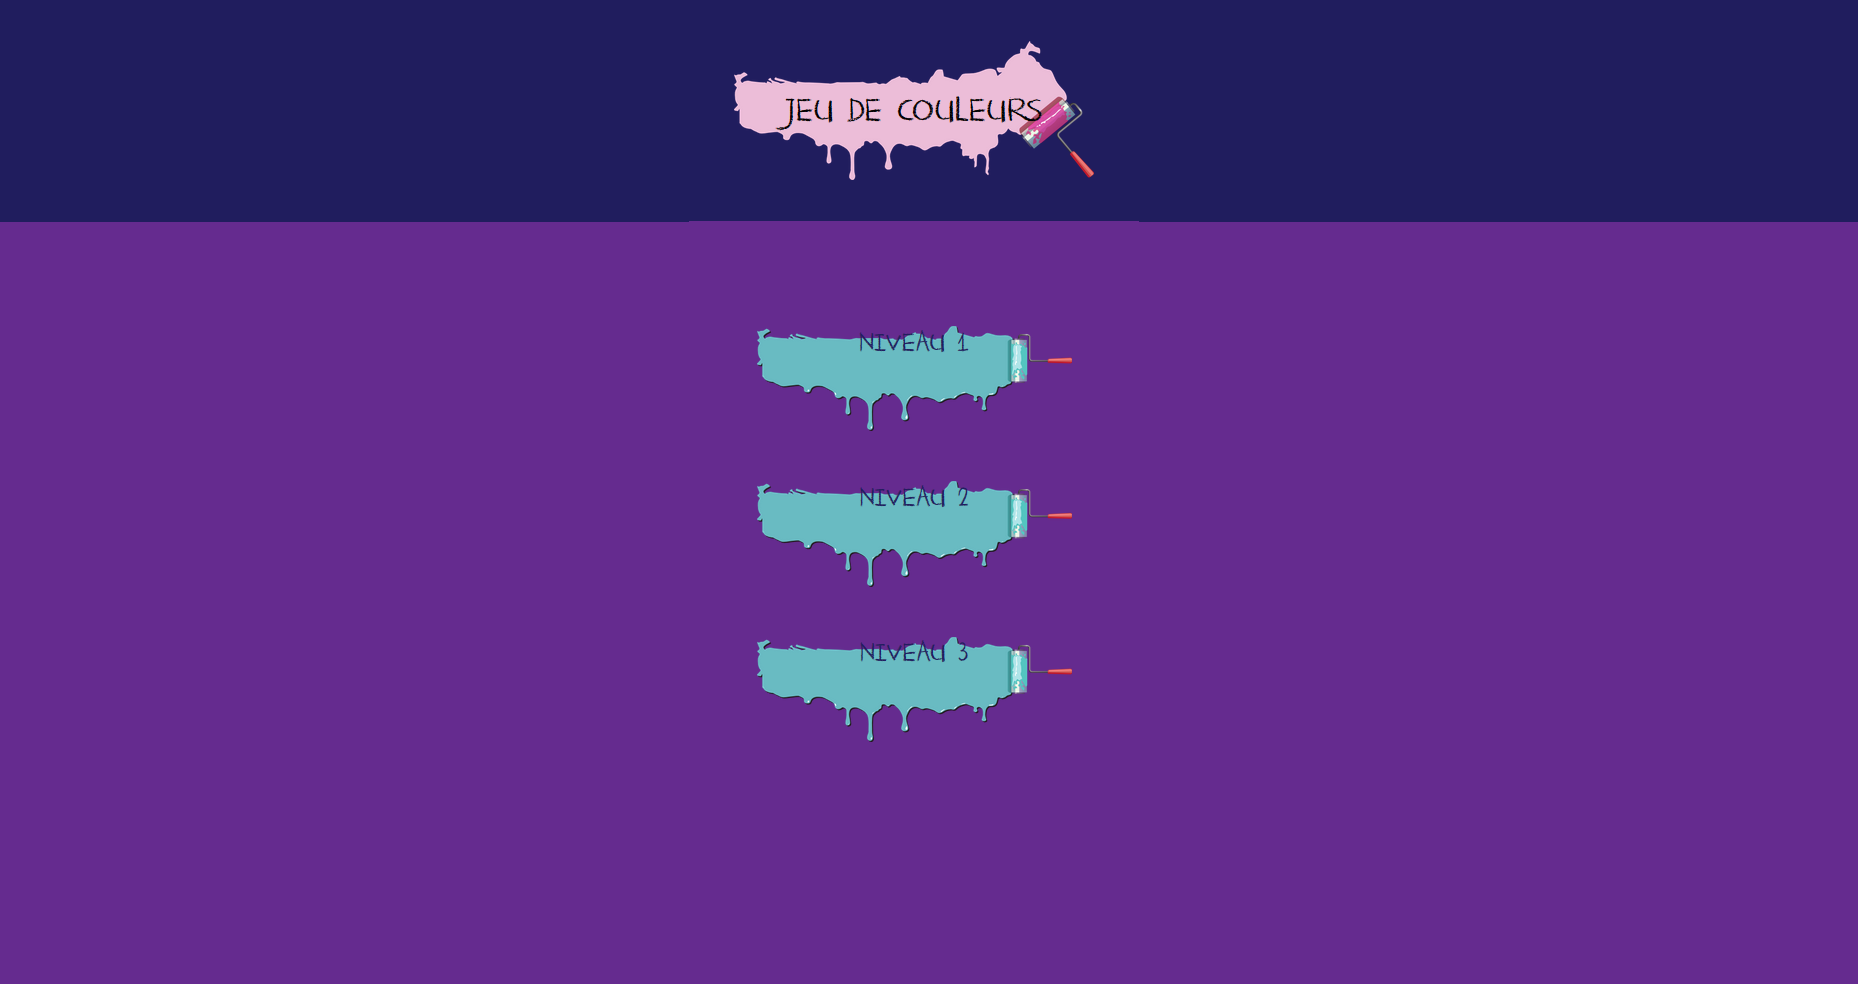
\includegraphics[width=0.28\textwidth]{2}
  \end{center}
  \vspace{-20pt}
  \caption{Menu difficilement lisible}
  \vspace{-10pt}
\end{wrapfigure}

Le menu principal, par exemple, n'utilise pas tout l'espace disponible, à certaines tailles d'écran il devient difficile de lire le menu. Moi-même qui n'ai qu'un léger problème de vue doit me forcer un peu pour lire le menu. La couleur, la taille ainsi que la police ont été très mal choisis. La couleur du texte est noir et repose sur un petit rectangle de couleur claire. Cependant tout le reste du fond est violet foncé. Il n'y a pas assez de contraste pour rendre le menu visible pour les malvoyants.\hfill\\

Dans les différents niveaux du jeu, il n'y a pas de grande faute majeur. Seulement de petit détail qui aurait pu être évité et ainsi amélioré l'expérience de l'utilisateur. Par exemple, le clic droit aurait pu être désactivé pour évité aux utilisateurs de faire un clic droit maladroit et se retrouver dans les menus du navigateur internet. Notons aussi que dans le niveau 2, il est possible de sortir les éléments de l'écran. Sur tablette, en faisant un mauvais mouvement, on peux donc se retrouver avec un élément hors de l'écran, le jeu en devient donc figé et il n'y a plus de solution au jeu.\\

\begin{wrapfigure}{r}{5cm}
\vspace{6pt}
\centering
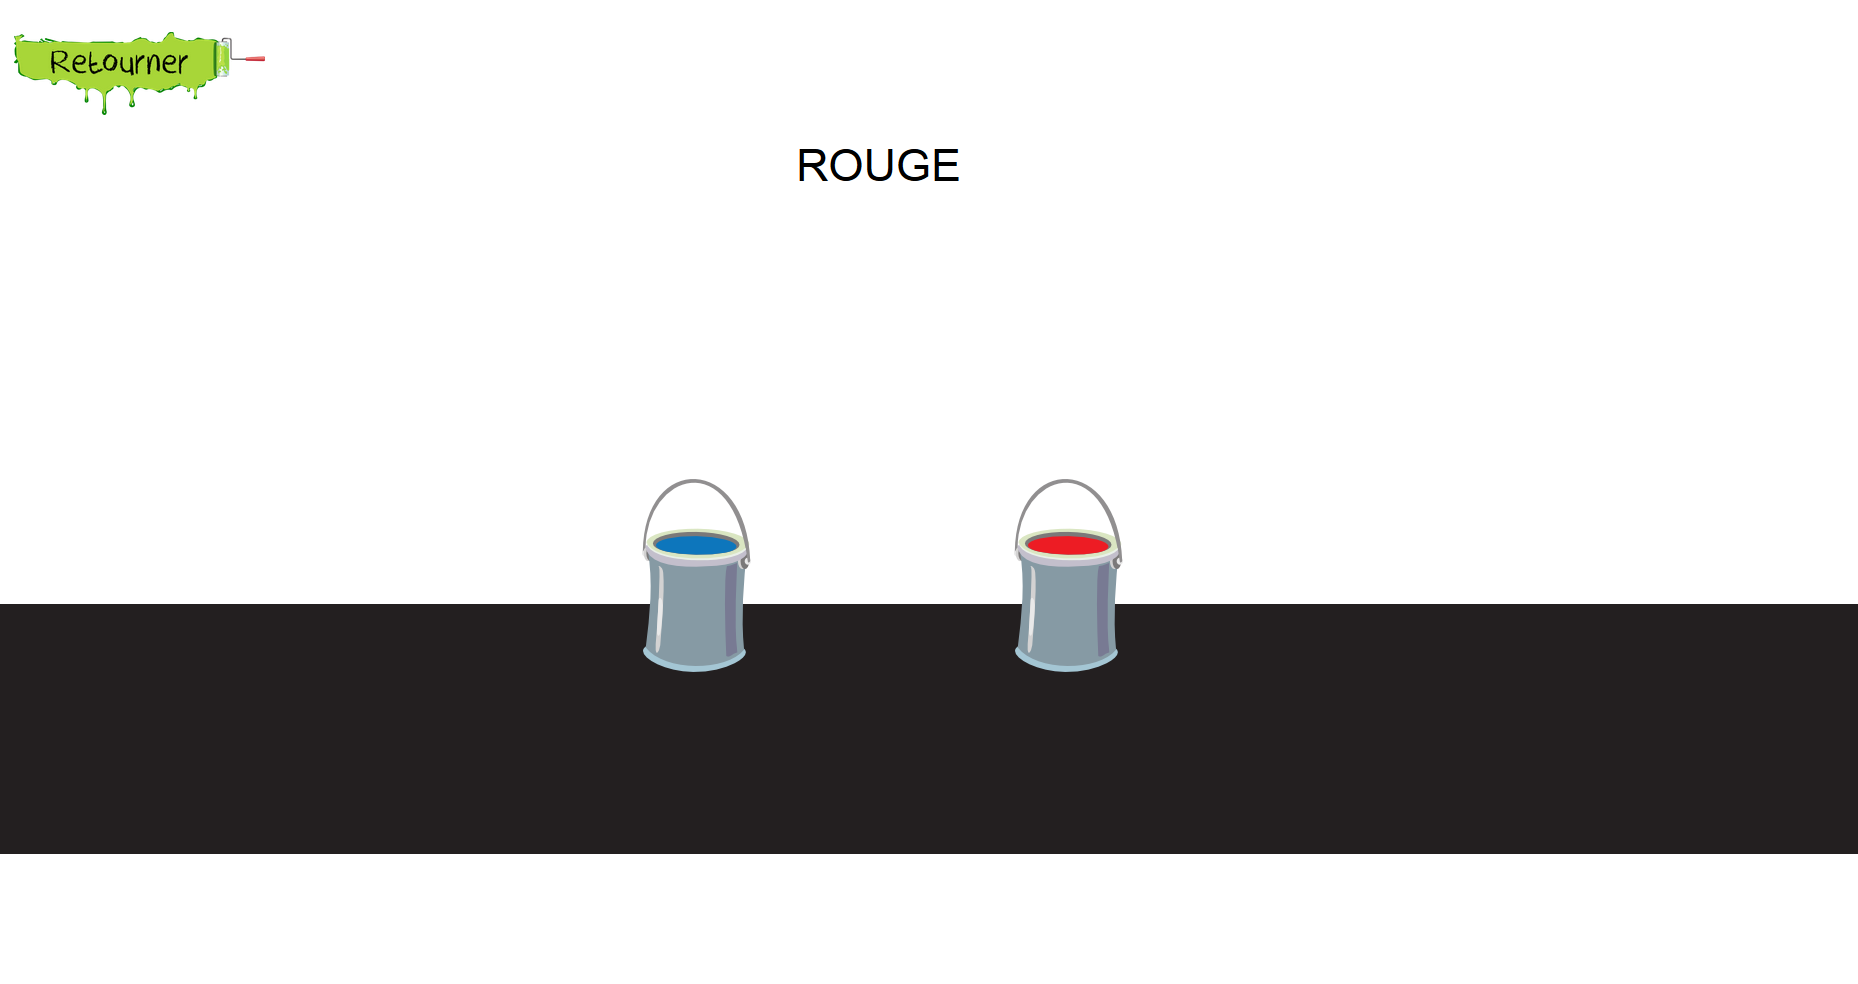
\includegraphics[width=5cm]{6}
\end{wrapfigure}

Sur le niveau 3, il y a un gros problème d'interférence. Nous sommes en plein dans l'effet Stroop. Cette notion du domaine psychologique précise que notre temps de réaction et pourcentage d'erreurs augmentent lorsqu'il y a des informations à filtrer. Inconsciemment, notre cerveau va lire la couleur affiché puis lire le mot. La couleur de ce niveau est marqué en noir. L'utilisateur va donc toujours penser à la couleur du texte en premier. Ensuite, l'utilisateur lira le mot et comprendra qu'il faut prendre tel ou tel autre couleur.
\vspace{0.5cm}\\

Il n'est pas si évident de lire le nom d'une couleur écrite avec une couleur différente. Il aurait mieux fallut associer la couleur du texte à la couleur écrite. Par exemple, une amélioration possible serait d'écrire en rouge, le mot rouge.\\

Sur le niveau 1, il y a aussi un petit problème. J'ai fait testé ce jeu à plusieurs personnes de mon entourage et elles ont toutes réagi de la même manière. Elles ont commencé à cliquer sur les couleurs puis voyant que cela était sans effet, elles ont commencé à cliquer un peu partout sur l'écran. Puis lorsque l'animation se lance, elles ne comprennent pas ce qui se passe. Il apparait que le temps d'attente avant que l'animation se lance est trop long. Il aurait peut-être été plus judicieux de mettre un texte ou symbole invitant le joueur à attendre ou alors faire que l'animation se déclenche plus rapidement.\\

Il y a aussi un point négative dans l'ordre d'exécution des ressources. Comme on peux le voir sur l'image ci-dessous qui est une analyse sous Firebug, les scripts sont chargés avant les images. Pour améliorer ce point, il aurait fallu mettre les scripts à la fin dans le code HTML et non au départ. 

\begin{center}
\vspace{0.5cm}
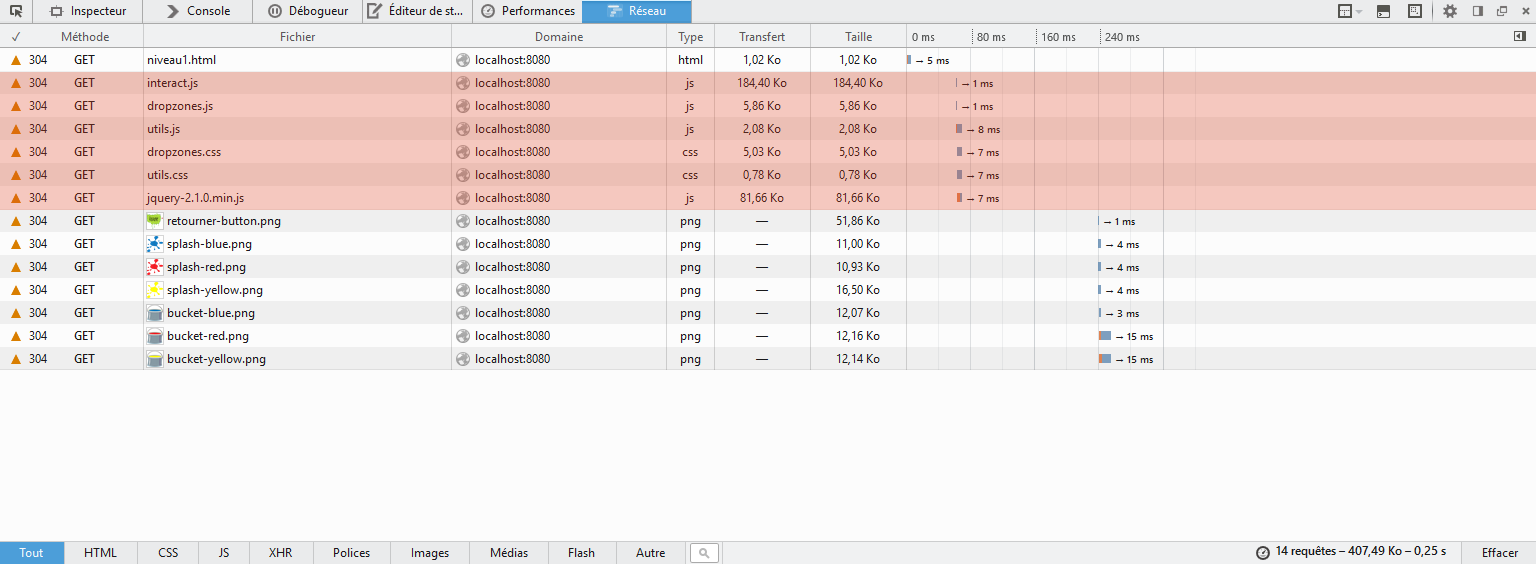
\includegraphics[width=\textwidth]{7}\\
\end{center}

Toujours dans Firebug, une autre chose est préoccupante. Sur l'image ci-dessous, on remarque que les FPS (Frames per second/Images par seconde) moyen ne sont qu'à 52. Pour un tel jeu, il est étonnant que ce chiffre ne soit pas égale à la fréquence de l'écran, soit 60 FPS. \\

On remarque que le jeu subit une chute de FPS à 3 FPS après 1,2 secondes de chargement de la page et jusqu'à 1,6 secondes. Plusieurs erreurs mineurs ralentissent le jeu ainsi que le "cycle collector" du navigateur, c'est à dire la recherche des ressources dans le dossier temporaire du navigateur. Pour un tel jeu où les ressources sont minuscules, il aurait été sans doute plus efficace de forcer le navigateur à ignorer cet étape.
\begin{center}
\vspace{0.5cm}
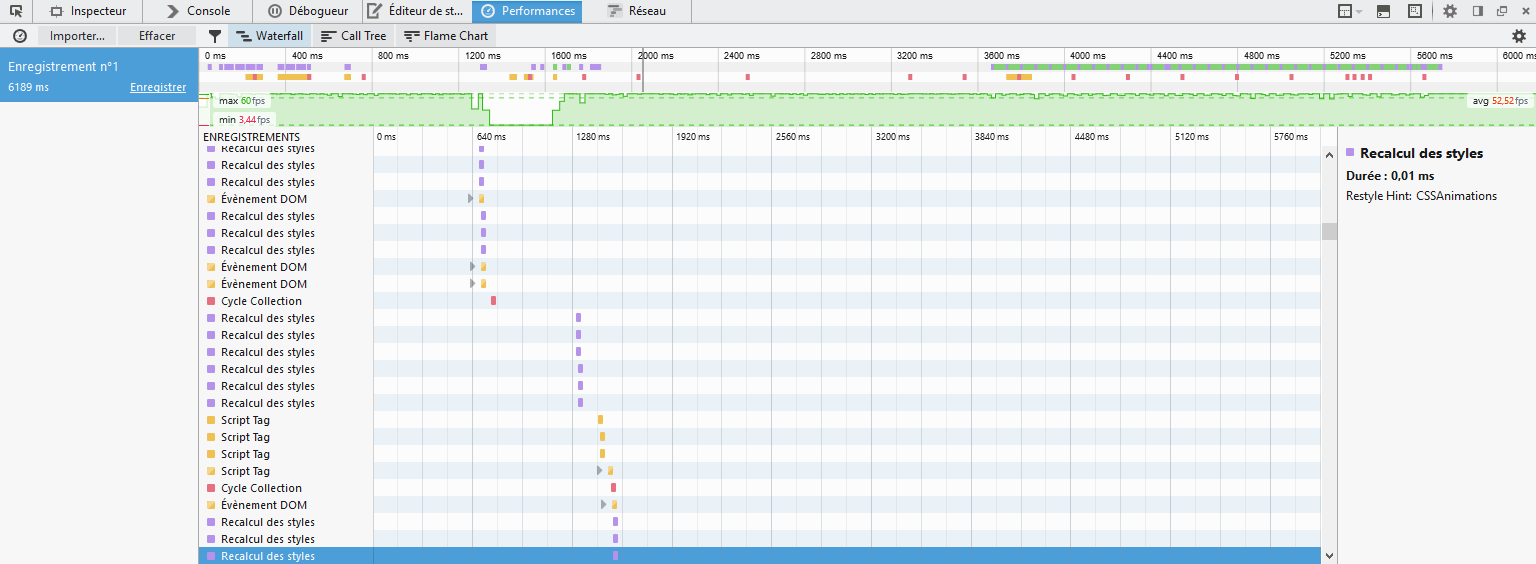
\includegraphics[width=\textwidth]{8}\\
\end{center}

\newpage

\section{Programmation}

\hspace*{0.6cm}Du coté programmation, il y a là aussi plusieurs problèmes plus ou moins embêtant. Premièrement, un code finit ne devrais jamais contenir de code commenté, c'est une mauvaise pratique. Cela peut avoir de grave conséquence lors d'un d'une recherche de bug. Deuxièmement, le code contient du "dead code", c'est à dire du code qui ne sera jamais atteint ou qui ne servira jamais lu peut importe ce qu'il contient. Par exemple, dans le niveau 1, on retrouve une balise "script" vide et après la balise "html".

\vspace{0.4cm}
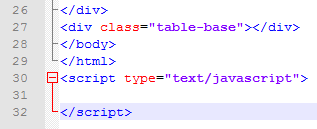
\includegraphics[width=0.40\textwidth]{9}\\

La seconde chose à noté est l'utilisation très mauvaise des attributs CSS. Cette mauvaise manipulation rend le jeu inadapté sur certains écran.\\
\begin{wrapfigure}{r}{5cm}
\vspace{-13pt}
\centering
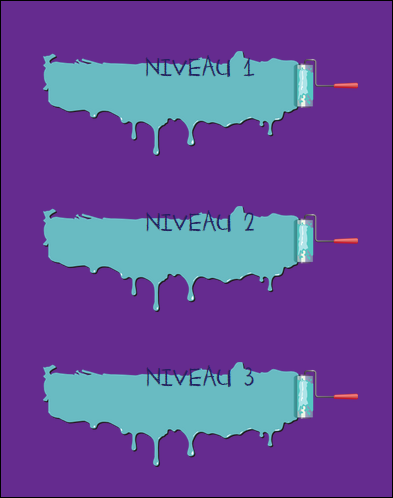
\includegraphics[width=5cm]{1}
\caption{\textit{à certaines dimensions d'écrans, le texte sort du graphisme.}}
\end{wrapfigure}
Il s'agit là d'une des permières erreurs qui m'a simplement sauté aux yeux. Mon écran étant relativement grand par rapport à la moyenne, je remarque généralement très rapidement si un site ou un jeu s'adapte ou non à l'écran de l'utilisateur. Ici, comme on peux le voir sur l'image de droite, le jeu ne s'adapte pas du tout à tous les utilisateurs. L'erreur a été assez simple à trouver, il s'agit d'une incompréhension des étudiants sur l'attribut CSS "padding" et "margin". Il fallait tout simplement utiliser le padding à la place du margin dans les balises divisions "option". Sans cela, la balise "div" qui était contenue dans la balise "a" se retrouvait tout simplement à une taille différente de la balise "a" qui l'entourait. Cette erreur se reproduit sur les 3 liens vers les différents niveaux.\\

Il y a aussi une utilisation très mauvaise des balises "div" ou une méconnaissance de certains attributs fondamentales de CSS.\\


\begin{wrapfigure}{r}{0.34\textwidth}
  \vspace{-20pt}
  \begin{center}
    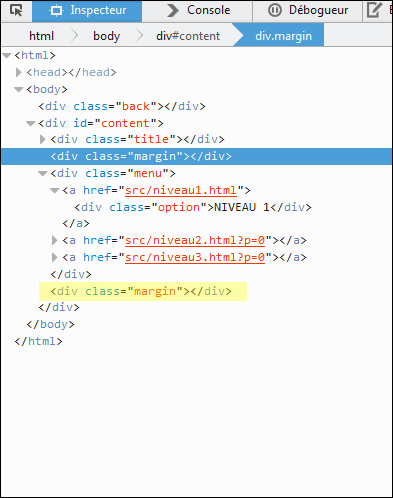
\includegraphics[width=0.33\textwidth]{3}
  \end{center}
  \vspace{-20pt}
  \caption{Le groupe de développeurs}
  \vspace{-10pt}
\end{wrapfigure}


Le rectangle jaune sur l'image de gauche pointe sur un problème sérieux de programmation, les élèves responsables de ce code ont utilé des balises "div" pour effectuer des marges et ainsi réaliser le positionnement de leurs éléments HTML. Ceci est considéré comme une très mauvaise pratique. Pour réaliser le positionnement, il est plus intéressant d'utiliser les attributs CSS tels que "position","display","float","margin","padding"... On peux de plus noté que les élèves n'ont aussi pas respecté les normes du W3C (World Wide Web Consortium). Il est non conforme d'englobé une balise "block" comme une "div" dans une balise "inline" comme un "a". Pour regler ce problème, il fallait soit faire de la balise "div" un lien vers la page en utilisant JavaScript ou alors transformer l'attribut "display" de la balise "div" en "inline" ou "inline-block".\\

\newpage
\section{Amélioration}

\hspace*{0.6cm}J'ai déjà proposé aux travers de mon document plusieurs améliorations, je vais donc les regrouper ici et en complétant cette liste avec d'autres idées :\\
\begin{itemize}
  \item Mettre un bouton ou une indication que le jeu au niveau 1 montre le gameplay et qu'il n'y a rien à faire.
  \item Améliorer la visibilité du texte au menu
  \item Mettre le texte de la même couleur que celle écrite dans le niveau 3.
  \item Désactiver le clique droit pour éviter que l'utilisateur ne rentre dans les menus de son navigateur.
  \item Mettre une limite au déplacement possible des éléments dans le niveau 2, sinon on peux bloquer le jeux en sortant un élément de l'écran.
  \item Rendre le jeu compatible avec tous les navigateurs (Le jeu ne fonctionne pas sous Safari)
  \item Ajouter les couleurs complémentaires (rose,orange..)
  \item Mettre une option permettant d'ajouter ou d'enlever des pots de peintures.
\end{itemize}


\end{document}
